\documentclass[a4paper,12pt,russian]{report}
\usepackage[utf8]{inputenc}
\usepackage[T2A]{fontenc}
\usepackage{amsmath}
\usepackage{listings}
\usepackage{xcolor}
\usepackage{tabularx}
\usepackage{geometry}
\usepackage{titlesec}
\usepackage{graphicx}
\usepackage[font=small,labelfont=bf]{caption}
\usepackage{indentfirst}

\newcommand{\insertInstitute}{
  Институт компьютерных наук и технологий\linebreak
  Высшая школа «Киберфизических систем и управления»
}
\newcommand{\insertTitle}{Расчетно-графическая работа\par по дисциплине «Технологии современных материалов»\par \textbf{Материалы, используемые для изготовления труб}}
\newcommand{\insertAuthor}{С. А. Новиков}
\newcommand{\insertAuthorPosition}{студент гр 13532/1}
\newcommand{\insertVerifier}{Т. А. Итс}
\newcommand{\insertVerifierPosition}{доцент, к.т.н.}

\newcommand{\sectionbreak}{\clearpage}
\newcommand{\subsectionbreak}{\clearpage}

\graphicspath{ {./images/} }

\sloppy

\linespread{1.3}
\definecolor{lightgray}{gray}{0.95}
\renewcommand{\contentsname}{Содержание}
\renewcommand{\thesection}{\arabic{section}}
\newgeometry{left=3cm,right=2cm,top=2cm,bottom=2cm}
\setlength{\parindent}{1.25cm}
\lstset{
  backgroundcolor=\color{lightgray},
}


\begin{document}
\pagenumbering{gobble}
\begin{center}
  Министерство науки и высшего образования РФ\linebreak
  Санкт-Петербургский политехнический университет\linebreak
  Петра Великого\linebreak
  \insertInstitute\linebreak
\end{center}
\vspace{1.5cm}
\begin{tabularx}{\textwidth}{Xr}
  УДК $\rule{4cm}{0.15mm}$ & УТВЕРЖДАЮ \\
                           & $\rule{5cm}{0.15mm}$ \\
                           & $\rule{5cm}{0.15mm}$ \\
                           & $\rule{5cm}{0.15mm}$ \\
                           & «$\rule{0.8cm}{0.15mm}$» $\rule{2cm}{0.15mm}$ $\rule{1.1cm}{0.15mm}$ г. \\
\end{tabularx}
\vspace{1.5cm}
\begin{center}
  \insertTitle\par
\end{center}
\vspace{1.5cm}
\begin{tabularx}{1\textwidth}{Xll}
  \textbf{Выполнил:}    & & \\
  \insertAuthorPosition & $\rule{3.5cm}{0.15mm}$ & \insertAuthor \\
                        & подпись, дата & \\
  \textbf{Проверил:}      & & \\
  \insertVerifierPosition & $\rule{3.5cm}{0.15mm}$ & \insertVerifier \\
                          & подпись, дата & \\
\end{tabularx}
\vfill
\begin{center}
  Санкт-Петербург $\rule{1.1cm}{0.15mm}$ г.
\end{center}


\newpage
\pagenumbering{arabic}
\setcounter{page}{2}

\tableofcontents

\section*{Реферат}

\noindent Отчет 15 с., 2 рис., 1 табл., 5 источник. \\
МАТЕРИАЛ, ТРУБЫ, ВОДОПРОВОД. \\
Объектом исследования является изучение существующих материалов для изготовления водопроводных труб. \\

\section{Введение}

Трубы - полое цилиндрическое или профильное изделие. Основными характеристиками труб являются: условный проход, наружный диаметр, толщина стенки и масса одного погонного метра трубы.

В современном мире мы часто забываем о значении в нашей жизни тех или иных предметов, которые, между тем, продолжают играть не маловажную роль в жизни современных мегаполисов. Именно такие роли отведены трубам. Казалось бы, что может быть проще труб? Мы ведь так к ним уже привыкли. Привыкли, легонько повернув кран получать воду, а не таскать ее ведрами с ближайших колодцев, привыкли не топить печь, чтоб согреться в зимние месяцы, теперь тепло в дом несут батареи, теперь нам костры заменяют газовые плиты, да и много всего принесли в нашу жизнь трубы.
Трубы, основной идеей конструкции которых человека снабдила сама природа, представляют собой один из старейших конструктивных элементов, вне всякого сомнения. Когда человек впервые смастерил и применил трубу - теперь не представляется возможным установить, так как самые первые трубы изготавливали из малопрочных материалов (тростник, бамбук, дерево).
Далее посмотрим историю развития труб из различных материалов.

\section{Материалы для изготовление труб}

\subsection{Металлические трубы}

Наиболее древняя металлическая труба, сохранившаяся до наших дней, изготовлена из меди. Найдена она было в Египте. Это часть водостока древнеегипетского храма. Ее точно установленный возраст составляет 4700 лет, и храниться она в Городском музее Западного Берлина. Она изготовлена из кованного медного листа. Кромки соединены между собой в нахлестку кузнечной сваркой. Для защиты тонкостенной трубы от механических повреждений ее уложили в вырубленный в камне желоб и сверху залили известковым мертелем. Трубы изготавливали и в древнем Риме. Римляне применяли литые трубы из бронзы и трубы из металлического листа с паяным швом. Из литых металлических листов формовали трубы диаметром от 25 до 300мм. И что интересно, римляне уже тогда применяли своего рода стандартизацию, которую использовали для регламентации ширины металлического листа. Продольный шов выполняли различными способами. Чаще всего трубы грушевидного сечения накрывали U-образной свинцовой полосой и затем запаивали оловянно-свинцовым припоем. Иногда встречались паяные соединения встык или внахлестку, и даже стыки с желобчатым изгибом кромок, уплотненные смазкой. Однако такие трубы затем замуровывали в каменную кладку, чтобы сохранить их герметичность.
Стальные трубы впервые изготовил А.Пенспен. Произошло это более 125 лет назад. Вначале это были трубы с кузнечной сваркой, а братья Маннесман изобрели бесшовную трубу спустя несколько десятилетий после появления на свет "детища" Пенспена.  Далее были разработаны различные технологические процессы производства как сварных, так и бесшовных труб.

\begin{figure}[!htb]
  \centerline{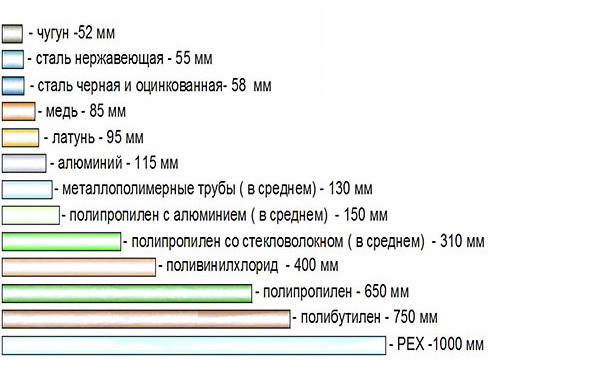
\includegraphics[width=0.9\textwidth]{50}}
  \caption{Диаграмма линейного удлиннения 100 м трубы при нагреве на 50 C}
  \label{graph:50}
\end{figure}

\subsection{Чугунные трубы}

Первые литые чугунные трубы (из серого чугуна)  для водопроводов не имели внутренних и внешних покрытий и устанавливались в трубопроводах в том виде, в котором они приходили из литейных цехов после очистки. Было предложено использование битумных покрытий, и большинство труб из серого чугуна, продававшихся для использования в водоснабжении после 1860 года, поступали с внешним и внутренним битумным покрытиями, наносившимися методом погружения в горячий расплав.  В 1922 г. ACIPCO выпустила первую трубу из серого чугуна с внутренним цементно-песчаным покрытием, которая была установлена в системе водоснабжения г. Чарльстон, Южная Каролина.

\subsection{Пластиковые трубы}

Первое поколение пластиковых труб появилось в 30-х годах ХХ века. Первые разработки не носили серийный характер и предназначались для монтажа частных, малогабаритных коммуникационных разводок. В связи с этим, модельный ряд первых пластиковых труб был весьма ограничен. Трубопроводы создавались с помощью фитингов, присоединяемых посредством специального клея.

50-е годы прошлого века подарили миру новый вид пластиковых изделий – полиэтиленовые трубы. Новый материал, поначалу, не мог похвастаться высокой прочностью и устойчивостью к высоким температурам. Самым главным преимуществом первых полиэтиленовых труб была высокая устойчивость к отрицательным температурам (нормальное функционирование оставалось возможным до отметки в 20 градусов ниже нуля). В связи с этим, монтаж полиэтиленовых трубопроводов мог осуществляться даже в условиях «русской» зимы. Основная область применения первых полиэтиленовых труб – это системы холодного водоснабжения невысокого давления. Однако, с появлением технологии молекулярного сшивания, разработанной ведущими химиками в 70-х годах, новые ПВД и ПНД трубы приобрели широкую популярность в качестве материалов, предназначенных для создания высокоэффективных коммуникационных сетей. Сшитый полиэтилен обладает высокой прочностью и стойкостью к высоким температурным воздействиям. Традиционно, отдельные ПНД и ПВД трубы соединяются в единую конструкцию с помощью монолитных латунных или более легких полипропиленовых фитингов. Современная промышленность выпускает несколько модификаций полиэтиленовых труб, различающихся методом изготовления: с использованием высокого (ПВД) или низкого давления (ПНД). Полиэтиленовые трубы, выполненные по технологии сшивания молекул, успешно используются в системах горячего водоснабжения, а изделия, имеющие специальный «кослородозапирающий» слой, применяются для создания отопительных сетей.

\begin{figure}[!htb]
  \centerline{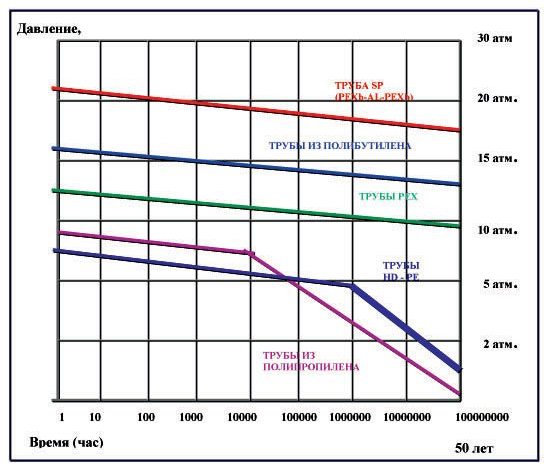
\includegraphics[width=1\textwidth]{95}}
  \caption{График соотношения долговечности и внутреннего давления}
  \label{graph:95}
\end{figure}

\subsection{Металлополимерные трубы}

Металлополимерные трубы являются представителем следующего поколения и имеют одну из самых сложных конструкций. Каждая металлопластиковая труба состоит из пяти слоев: основная полиэтиленовая труба, прослойка из специального клея, тонкая алюминиевая фольга, новый слой клея и полиэтиленовое защитное покрытие. При этом толщина алюминиевой фольги составляет всего десятые доли миллиметра. В связи со сложностью конструкции, промышленностью выпускаются металлополимерные трубы, имеющие диаметр не больше 40 миллиметров, что существенно ограничивают их возможные области использования.

Полипропилен – это самый совершенный материал, относящийся к последнему поколению пластиковых изделий. Полипропиленовые трубы представляют собой диффузионный сплав, отличающийся высокой прочностью, температурной стойкостью и долговечностью. Используются для создания современных коммуникаций.

\subsection{Стеклянные трубы}

Стеклянные трубы благодаря высокой химической стойкости, гладкости поверхности и прозрачности с успехом соперничают с металлическими. В ряде областей (например, химическая и пищевая промышленность) их применение предпочтительнее. Пропускная способность стеклянных труб на 5-10\% выше, чем стальных при одинаковом диаметре. Основной недостаток стеклянных труб — хрупкость и низкая термостойкость (допустимый перепад температур 50° С). Стеклянные трубы используют как в вакуумных, так и в напорных (до 0,7 МПа) сетях.

\subsection{Стеклопластиковые трубы}

Стеклопластиковые трубы - изделие из композиционного материала. Стеклопластик представляет собой композиционный конструкционный материал, который сочетает в себе высокую прочность и относительно небольшую плотностью. В разных отраслях промышленности стеклопластик успешно конкурирует с традиционными материалами, такими как металлы и их сплавы, бетон, стекло, керамика, дерево и пр.

Для производства стеклопластиковых труб применяются различные типы связующего и армирующего материала, который определяет области их применения: эпоксидные (GRE), полиэфирные (GRP), винилэфирные и пр. Также, на сегодняшний день известно несколько способов производства стеклопластиковых труб, обусловленных областями применения и компанией-производителем. Это могут быть переодическая или непрерывная намотка или центробежное формование.

Основными преимуществами стеклопластиковых труб являются высокие удельные показатели прочности и жесткости,  химическая стойкость, сравнительно малый вес и долговечность. Такой набор характеристик сделал этот материал привлекательными для строительства трубопроводов различного назначения, а также обеспечил хорошую репутацию у строителей и эксплуататоров сетей.

Стеклопластиковые трубы успешно применяются в России начиная с середины XX века в областях связанных с транспортировкой нефти и газа. За последние 20 лет, стеклопластиковые трубы нашли широкое применение в сфере ЖКХ для строительства и реконструкции трубопроводов.

\subsection{Напорные железобетонные трубы}

Напорные железобетонные трубы производятся из тяжелого бетона методом виброгидропрессования. Предназначены трубы напорные для прокладки напорных трубопроводов и для транспортировки жидкости под давлением, с температурой не выше 40 градусов, и не агрессивной степенью воздействия на материал. Отличительным качеством железобетонных труб является простота их монтажа, достигаемая точностью изготовления и взаимно сопрягаемым между собой отшлифованными поверхностями железобетонного камня. Для обеспечения герметичности трубопровода, трубы железобетонные комплектуются резиновыми уплотнительными кольцами.

История появления железобетонных труб тесно связана с историей появления материала, из которых они сделаны. В этом году железобетон отмечает свой 138-й день рождения. Несмотря на свой солидный возраст, его возможности и в наши дни ещё далеко не исчерпаны. Между прочим, бетон появился ещё до Рождества Христова, но только в двадцать первом веке занял прочные позиции в строительстве, можно сказать без преувеличения, что он стал самым востребованным строительным материалом. Используемый уже на протяжении восьмисот лет древний "цементикум" практически не изменил. Его прочность до сих пор подтверждает отличное состояние виадуков и акведуков, построенных ещё в дохристианскую эпоху. Наверное, поэтому железобетонные трубы сейчас пользуются такой популярностью.

К началу XIX века традиционное каменное строительство исчерпало свои технические возможности. На его смену пришло строительство с использованием бетона. Благодаря своей пластичности и долговечности этот материал быстро завоевал популярность. В 1995 году на международном конгрессе была впервые сформулирована задача по созданию "высокоэффективного бетона" – этот термин придумали американцы, после чего он был взят на вооружение в Европе. Железобетонные трубы, в производстве которых будет использован такой бетон, способны справится с задачами по изоляции вод, загрязненных токсичными для человека материалами и веществами, образующимися в результате природных и техногенных катастроф, работы атомных электростанций и т.д.

Ведущие европейские специалисты считают, что бетон в новом веке получит своё "второе дыхание", и ему найдёт применение в новых областях строительства. Подтверждением этому может служить гонка в строительстве самых больших небоскрёбов, которая происходит в разных странах на разных континентах. Например, в Мельбурне (Австралия) планируется строительство 113-этажного здания высотой 560 м. Такие проекты возможно осуществить только с использованием высококачественных железобетонных конструкций.

\subsection{Асбестоцементные трубы напорные и безнапорные}

Асбестоцементные трубы в России с самого начала использовали в первую очередь для мелиоративных целей и по остаточному принципу – для прокладки канализации и питьевого водопровода. Для нужд коммунального хозяйства производимых асбестоцементных труб всегда не хватало, и в отрасли использовали металлические трубы. В 60 – 70-е гг. металлических труб стало не хватать для покрытия потребностей газовиков и нефтяников, но и тогда плановые органы страны и отечественные коммунальщики не переключили отрасль на использование асбестоцементных труб.
Асбестоцементные трубы, безусловно, имеют больше преимуществ в эксплуатации, чем металлические и полиэтиленовые. Асбестоцементные трубы стойки к агрессивным средам, не подвержены коррозии и не нуждаются в гидроизоляции. Поскольку трубы неэлектропроводны, по ним не проходят блуждающие токи, они не нуждаются в катодной защите, как металлические. В отличие от металлических, асбестоцементные трубы не отпотевают при транспортировке холодной воды. Из-за отсутствия коррозии внутренняя поверхность труб не «зарастает». . Низкая теплопроводность асбестоцемента делает особенно выгодным использование асбестоцементных труб для транспортировки горячей воды. Асбестоцементные трубы в 2-5 раз дешевле стальных, чугунных, пластмассовых и намного долговечнее металлических и пластмассовых труб.

\section{Анализ материалов}

\begin{table}[!htb]
\centering
\caption{Достоинства и недостатки материалов}
\label{table:compare}
\begin{tabular}{|p{8cm}|p{8cm}|}
  \hline
  Достоинства & Недостатки \\
  \hline
  \multicolumn{2}{|c|}{Сталь} \\
  Механическая прочность & Подверженность коррозии \\
  Относительная дешевизна & Неизбежное сужение просвета труб на холодной воде \\
                          & Образование гальванической пары с алюминием и медью \\
  \multicolumn{2}{|c|}{Оцинковка} \\
  Прочность & Высокая цена \\
  Поверхность не подвержена коррозии & \\
  \multicolumn{2}{|c|}{Медь} \\
  Отсутствие коррозии & Высокая цена \\
  Отсутствие отложений & Редкость в продаже \\
  \multicolumn{2}{|c|}{Металлопластик} \\
  Отсутствие коррозии & Выдерживают ограниченное количество циклов нагрева \\
  Легкость монтажа & \\
  \multicolumn{2}{|c|}{Полипропилен} \\
  Герметичность и надежность стыков & \\
  Прочные трубы & \\
  Аккуратный монтаж фитингов & \\
  \hline
\end{tabular}
\end{table}

\section{Список литературы}

\begin{enumerate}
  \item Производство труб / А. Коликов, Ю. Райков, Ю. Шевакин // Интермет Инжиниринг. - 2005. 268 с.
  \item Трубопровод [Электронный ресурс] — Режим доступа: URL: https://ru.wikipedia.org/wiki/Трубопровод
  \item Труба (изделие) [Электронный ресурс] — Режим доступа: URL: https://ru.wikipedia.org/wiki/Труба\_(изделие)
  \item Водоснабжение [Электронный ресурс] — Режим доступа: URL: https://ru.wikipedia.org/wiki/Водоснабжение
  \item Полимерные трубы [Электронный ресурс] — Режим доступа: URL: https://ru.wikipedia.org/wiki/Полимерные\_трубы
\end{enumerate}

\end{document}
